Relacionado a los resultados de cada uno de las ejecuciones del algoritmo, las Figuras \ref{fig:AG_1}, \ref{fig:AG_2} y \ref{fig:AG_3} muestran el proceso de convergencia, donde se puede observar que todas las ejecuciones convergieron en una solución óptima.

\begin{figure}[htbp]
	\centering
	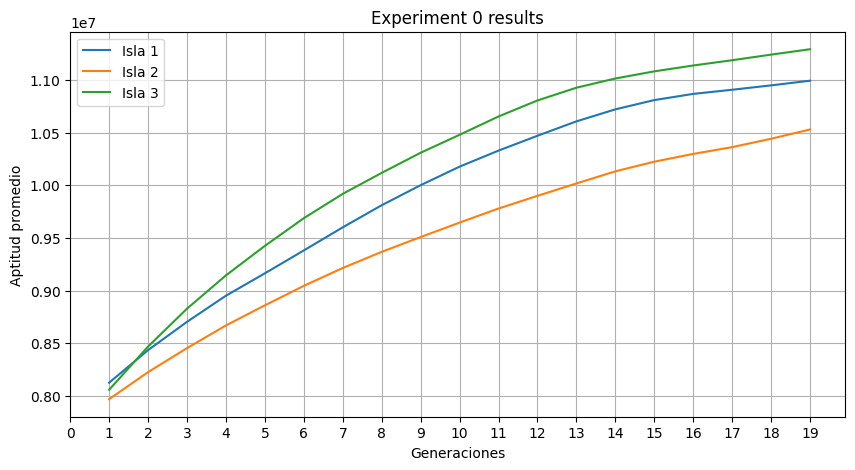
\includegraphics[width=0.6\textwidth]{experiment_0_results}
	\caption{Evolución de la aptitud de las islas en la primer ejecución del algoritmo.}
	\label{fig:AG_1}
\end{figure}

\begin{figure}[htbp]
	\centering
	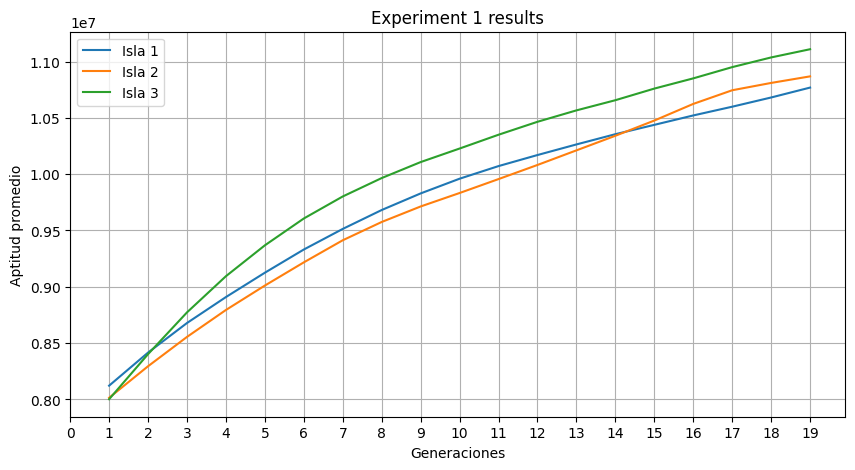
\includegraphics[width=0.6\textwidth]{experiment_1_results}
	\caption{Evolución de la aptitud de las islas en la segunda ejecución del algoritmo.}
	\label{fig:AG_2}
\end{figure}

\begin{figure}[htbp]
	\centering
	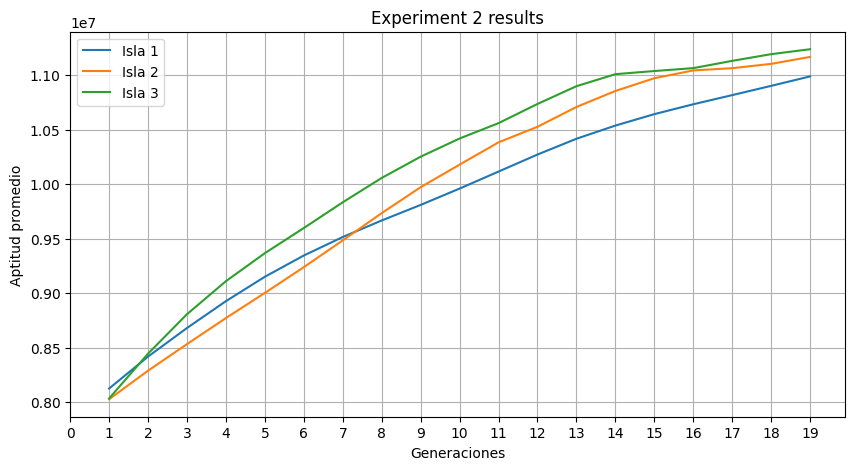
\includegraphics[width=0.6\textwidth]{experiment_2_results}
	\caption{Evolución de la aptitud de las islas en la tercer ejecución del algoritmo.}
	\label{fig:AG_3}
\end{figure}

\FloatBarrier
Relacionado a los resultados finales de cada ejecución, la Tabla \ref{tab:resultados} muestra mejor aptitud de cada una de las islas, así como su valor promedio del top 10.

\begin{table}[htbp]
\centering
\caption{Mejores aptitudes obtenidas en cada ejecución del algoritmo.}
\begin{tabular}{ccccccc}
\hline
\multirow{2}{*}{Experimento} & \multicolumn{2}{c}{Isla 1} & \multicolumn{2}{c}{Isla 2} & \multicolumn{2}{c}{Isla 3} \\ \cline{2-7} 
                             & Mejor        & Promedio    & Mejor        & Promedio    & Mejor        & Promedio    \\ \hline
Experimento 1                & 11,250,000   & 11,020,000  & 11,325,000   & 10,883,750  & 11,425,000   & 11,194,000  \\
Experimento 2                & 11,175,000   & 10,983,750  & 11,325,000   & 11,062,750  & 11,475,000   & 11,259,500  \\
Experimento 3                & 11,350,000   & 11,081,000  & 11,200,000   & 11,064,250  & 11,400,000   & 11,229,750  \\ \hline
\end{tabular}
\label{tab:resultados}
\end{table}